%!TEX root = /Users/patricpf/Documents/repos/Bauschule-Baustoffe/Unterlagen/05_Beton/02_Frischbetonkontrollen/Frischbetonkontrollen.tex
%!TEX program = lualatex

% !TEX program = lualatex
\documentclass[
    %answers,
    a4paper,ngerman,11pt, addpoints]{exam}

\usepackage[utf8]{inputenc}
%\usepackage[T1]{fontenc}
%\usepackage[ngerman]{babel}


\usepackage{polyglossia}
\setdefaultlanguage[variant = swiss]{german}
\usepackage{fontspec}
\setmainfont{Arial} % Bauschule CI Manual
\setsansfont{Arial} % Bauschule CI Manual


\usepackage[ a4paper,
 total={165mm,250mm},
 left=25mm,
 top=25mm,
 headsep=10mm
 %footsep=12mm
 %,showframe
  ]{geometry}

\usepackage{graphicx}
\usepackage{siunitx}
\usepackage{booktabs} % schöne Tabellen
\usepackage{float}
\floatplacement{figure}{H}
\usepackage{xcolor}
\usepackage{pdfpages}
\usepackage{enumitem}
\usepackage{mdframed} % Boxen
\usepackage{amsmath,amssymb}
\usepackage{tcolorbox}
\usepackage{lastpage} % For the total number of pages
\usepackage{gensymb}
\usepackage{xspace}
\usepackage{tabularx}
\usepackage{multicol}
\usepackage[
    version=3,
    arrows=pgf-filled,
]{mhchem} % für chemische Formeln
%\usepackage{microtype}
\usepackage{subfigure}
\usepackage[hidelinks]{hyperref}
\usepackage{cleveref}
\usepackage{luacode}
\usepackage{amsmath}
\usepackage{textcomp}


\sisetup{
  locale = DE,
  inter-unit-product = \ensuremath{{\cdot}},
  detect-all,
}

% Colors
\definecolor{blau_bauschule}{RGB}{22,65,148}
\CorrectChoiceEmphasis{\color{blau_bauschule}}
\SolutionEmphasis{\color{blau_bauschule}}

\setlength{\parindent}{0em} % Verhindert einrücken
\setlength\linefillheight{0.3in}


%% COMMMANDS
\author{Patrick Pfändler}
\newcommand{\dozent}{Patrick Pfändler}
\newcommand{\fach}{Baustoffe}


\newcommand{\punkte}[1]{%
    \begin{infobox}%
        #1
    \end{infobox}}%
\newcommand{\FinRes}[1]{\underline{\underline{#1}}}

\newmdenv[linecolor=black,backgroundcolor=gray!15,frametitle={Punktverteilung},leftmargin=1cm,rightmargin=1cm]{infobox}

\newcommand{\pagebreaksol}{
    \ifprintanswers
        \clearpage
    \else
        {}
    \fi
}

\newcommand{\pagebreakexam}{
    \ifprintanswers
        {}
    \else
        \clearpage
    \fi
}

\SolutionEmphasis{\color{blau_bauschule}}
\makeatletter%
\newcommand{\solutiontable}[1]{\ifprintanswers\begingroup\Solution@Emphasis#1\if@shadedsolutions%
            {\cellcolor{SolutionColor}}%
        \else%
        \fi\endgroup\else\phantom{#1}\fi}%
\makeatother%

\newcommand{\myNmm}[1]
{
    \sisetup{per-mode=symbol}
    \SI{#1}{\newton\per\mm\squared}
}

\renewcommand{\thequestion}{\fontsize{12pt}{2pt} \selectfont  \bfseries \arabic{question}}
\sisetup{per-mode=symbol}



%% Translation

\pointpoints{Punkt}{Punkte}
\bonuspointpoints{Bonuspunkt}{Bonuspunkte}
\renewcommand{\solutiontitle}{\noindent\textbf{Lösung:}\enspace}
\chqword{Frage}
\chpgword{Seite}
\chpword{Punkte}
\chbpword{Bonus Punkte}
\chsword{Erreicht}
\chtword{Gesamt}
\hpword{Punkte:}
\hsword{Ergebnis:}
\hqword{Aufgabe:}
\htword{Summe:}


\renewcommand{\questionshook}{%
  %\setlength{\leftmargin}{0pt}% removes the indentation from the left
  \setlength{\labelwidth}{1.25cm}% adjusts label width
  \setlength{\itemindent}{0cm}% aligns the start of the item with the above
  \setlength{\labelsep}{0.25cm}% space between the label and the item text
}




%% header and footer
\pagestyle{headandfoot}
\firstpageheadrule
\runningheadrule

% Adjust the font size for the header
\firstpageheader{\fontsize{9}{11}\selectfont\fach}{}{\fontsize{9}{11}\selectfont\dozent \\ \blattname}
\runningheader{\fontsize{9}{11}\selectfont\fach}{}{\fontsize{9}{11}\selectfont\dozent \\ \blattname}

% Adjust the font size for the footer
\firstpagefooter{
\includegraphics[width=2.5cm]{bauschule-logo-5cm.png}}{}{\fontsize{9}{11}\selectfont\thepage\,/\,\pageref{LastPage}}
\runningfooter{
\includegraphics[width=2.5cm]{bauschule-logo-5cm.png}}{}{\fontsize{9}{11}\selectfont\thepage\,/\,\pageref{LastPage}}


%% header and footer

\pagestyle{headandfoot}
\firstpageheadrule
\runningheadrule
\firstpageheader{\fontsize{9pt}{2pt}\selectfont\fach}{}{\fontsize{9pt}{2pt}\selectfont\dozent \\ \blattname}
\runningheader{\fontsize{9pt}{2pt}\selectfont\fach}{}{\fontsize{9pt}{2pt}\selectfont\dozent \\ \blattname}
\firstpagefooter{
\includegraphics[width=2.5cm]{bauschule-logo-5cm.png}}{}{\fontsize{9pt}{2pt}\selectfont\thepage\,/\,\numpages}
\runningfooter{
\includegraphics[width=2.5cm]{bauschule-logo-5cm.png}}{}{\fontsize{9pt}{2pt}\selectfont\thepage\,/\,\numpages}

\usepackage{siunitx}

\sisetup{
  locale = DE,
  inter-unit-product = \ensuremath{{\cdot}},
  detect-mode,             % Use the surrounding text font mode
  detect-family,           % Use the surrounding text font family
  detect-weight,           % Use the surrounding text font weight
  mode = text              % Ensure that numbers and units are typeset in text mode
}

% Setzen des Blattnamens
\newcommand{\blattname}{Frischbetonkontrollen}


%\printanswers
\begin{document}
\section*{\blattname}
Die Konsistenz des Frischbetons bestimmt die Verarbeitbarkeit des Betons. Sie beschreibt neben dem inneren Zusammenhalt des Frischbetons wichtige Eigenschaften wie das Fliessverhalten, die Entmischungsneigung und die Glättbarkeit. Von der Konsistenz des Frischbetons hängt wesentlich ab, mit welchem Aufwand er sich auf der Baustelle fördern, einbringen und verdichten lässt. In der Schweiz werden für die Prüfung der Konsistenz vor allem die folgenden Verfahren eingesetzt:

\begin{itemize}
	\item Ausbreitmass
	\item  Verdichtungsmass nach Walz 
	\item Setzmass (Slump)
\end{itemize}


\subsection*{Ausbreitmass}
Das Ausbreitmass beschreibt quantitativ das Ausbreitvermögen von Frischbeton auf einer flachen Platte, die aus festgelegter Höhe auf einen Rahmen fallengelassen wird \cref{fig:BestimmungAusbreitmass}. 


\begin{figure}[h!bt]
	\centering
	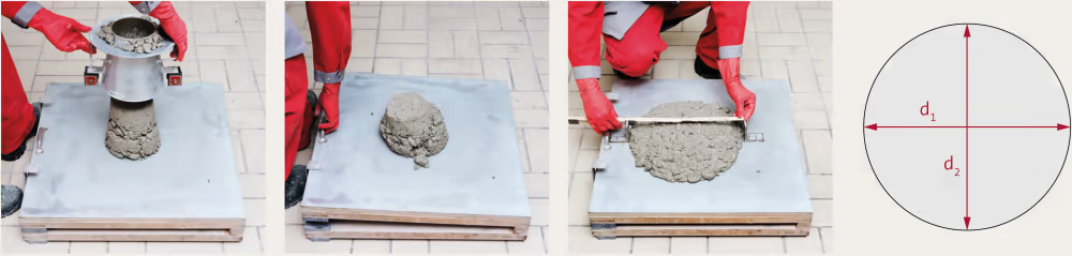
\includegraphics[width=1.0\linewidth]{Bilder/Ausbreitmass.png}
	\caption{Bestimmung des Ausbreitmasses gemäss der Norm SN EN 13350-5. (aus www.holcimpartner.ch)}
	\label{fig:BestimmungAusbreitmass}
\end{figure}

\begin{equation}
	f = \dfrac{d_1+d_2}{2}
	\label{eq:Ausbreitmass}
\end{equation}


\subsubsection*{Bestimmung des Ausbreitmasses}

\begin{enumerate}
    \item Sicherstellen, dass die Prüfgeräte den normativen Vorgaben entsprechen.
    \item Ausbreitmasstisch auf ebene, horizontale, nicht federnde Unterlage stellen.
    \item Ausbreittisch, Konusinnenseite und alle Geräte feucht abwischen.
    \item Frischbeton mit Schaufel in zwei gleich hohen Lagen in den Konus einfüllen.
    \item Jede Lage mit 10 Stössen des Holzstampfers verdichten.
    \item Abziehen der Betonoberfläche bündig zur Konusoberfläche mit Stampfer und Reinigen der Tischplatte rund um den Konus.
    \item 30 Sekunden nach Abstreichen des Betons ist der Konus sorgfältig und langsam innerhalb von 3–6 Sekunden vertikal hochzuziehen.
    \item Tischplatte bis zum Anschlag heben und frei fallen lassen, Dauer je Vorgang: 2–5 Sekunden, Anzahl Wiederholungen: 15. Dabei den Tisch durch Stehen auf den dafür vorgesehenen Trittblechen fixieren.
    \item Grössten Durchmesser des entstandenen Kuchens in zwei Richtungen $d_1$ und $d_2$ parallel zu den Tischkanten in Millimeter messen.
    \item Berechnen des Ausbreitmasses aus den beiden Messwerten mit Hilfe von  \cref{eq:Ausbreitmass}.  Das Ergebnis wird auf die nächsten 10 mm gerundet.
\end{enumerate}


\subsection*{Verdichtungsmass}
Das Verdichtungsmass wird als Volumenänderung erfasst und beschreibt quantitativ die Verdichtbarkeit eines Frischbetons, wenn dieser vibriert wird. Die Bestimmung des Verdichtungsmasses nach Walz (c) wird in der Norm SN EN 12350-4 definiert und ist in \cref{fig:BestimmungVerdichtungsmass} dargestellt.

\begin{equation}
	f = \dfrac{400}{400-c}
	\label{eq:Verdichtungsmass}
\end{equation}


\begin{figure}[h!bt]
	\centering
	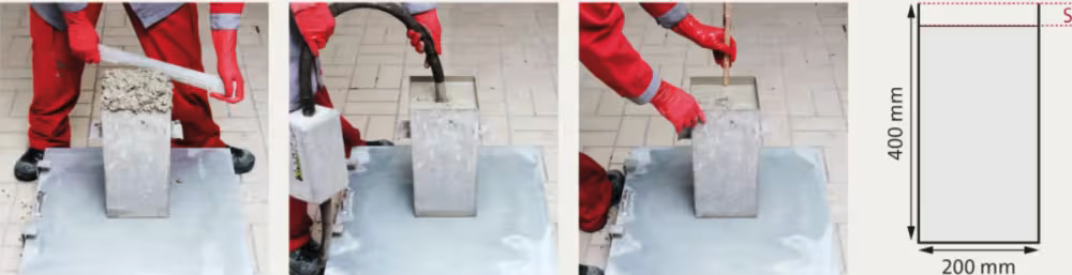
\includegraphics[width=1.0\linewidth]{Bilder/Verdichtungsmass}
	\caption{Bestimmung des Verdichtungsmasses nach Walz gemäss der Norm SN EN 12350-4. (aus www.holcimpartner.ch)}
	\label{fig:BestimmungVerdichtungsmass}
\end{figure}



\subsubsection*{Bestimmung des Verdichtungsmasses}

\begin{enumerate}
    \item Sicherstellen, dass die Prüfgeräte den normativen Vorgaben entsprechen.
    \item Behälter innen feucht abwischen und auf feste, ebene Unterlage stellen.
    \item Mit der Kelle abwechselnd über alle vier Kanten des Behälters Frischbeton lose einfüllen.
    \item Den überstehenden Beton mit einem Abstreich-Lineal in einer Sägebewegung entfernen (dabei ein Verdichten des Betons vermeiden).
    \item Beton mit einem Rütteltisch oder einem Innenrüttler verdichten bis keine Volumenverringerung mehr festzustellen ist.
    \item An jeder Seite des Behälters ist der Abstand zwischen der Oberfläche des verdichteten Betons und der Oberfläche des Behälters $s_1$ bis $s_4$ auf $1$ mm genau zu messen und der Mittelwert ($s$) zu bilden.
    \item Berechnen des Verdichtungsmasses aus dem Mittelwert mit \cref{eq:Verdichtungsmass}. Das Ergebnis wird auf zwei Dezimalstellen gerundet.
\end{enumerate}

\clearpage
\subsection*{Setzmass}
Das Setzmass beschreibt quantitativ das selbständige Absetzen des Frischbetons (siehe \cref{fig:BestimmungSetzmass}). Die Bestimmung des Setzmasses ($h$) wird in der Norm SN EN 12350-2 definiert.

\begin{figure}[h!bt]
	\centering
	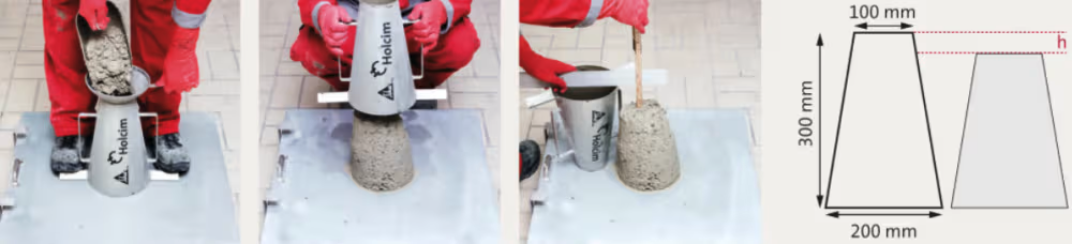
\includegraphics[width=1.0\linewidth]{Bilder/Setzmass}
	\caption{Bestimmung des Verdichtungsmasses nach Walz gemäss der Norm SN EN 12350-4. (aus www.holcimpartner.ch)}
	\label{fig:BestimmungSetzmass}
\end{figure}


\subsubsection*{Bestimmung des Setzmasses}

\begin{enumerate}
    \item Sicherstellen, dass die Prüfgeräte den normativen Vorgaben entsprechen.
    \item Innenfläche des Kegelstumpfs und Bodenplatte feucht abwischen.
    \item Frischbeton in drei gleich hohen Lagen einbringen, ohne den Kegelstumpf zu verschieben.
    \item Jede Schicht mit 25 Stössen des Stampfers verdichten. Dabei sind die normativen Vorgaben zur Durchführung zu beachten.
    \item Vor dem Füllen und Verdichten der obersten Schicht den Beton über die Form hinaus füllen.
    \item Den überstehenden Beton nach dem Verdichten der obersten Schicht mit dem Stahlstab bündig abstreichen und Unterlage reinigen.
    \item Kegelstumpf gleichmässig (ohne Drehen) senkrecht innerhalb von 2 bis 5 Sekunden hochziehen. Der gesamte Vorgang vom Beginn des Einfüllens bis zum Hochziehen der Form ist innerhalb von 150 Sekunden durchzuführen.
    \item Messen des Setzmasses ($h$) auf \SI{10}{\mm} genau, indem die Differenz zwischen der Höhe der Form und dem höchsten Punkt des abgesetzten Probekörpers bestimmt wird.
\end{enumerate}



 











\end{document}